%%%%%%%%%%%%%%%%%%%%%%%%%%%%%%%%%%%%%%%%%
% University Assignment Title Page 
% LaTeX Template
% Version 1.0 (27/12/12)
%
% This template has been downloaded from:
% http://www.LaTeXTemplates.com
%
% Original author:
% WikiBooks (http://en.wikibooks.org/wiki/LaTeX/Title_Creation)
%
% License:
% CC BY-NC-SA 3.0 (http://creativecommons.org/licenses/by-nc-sa/3.0/)
% 
% Instructions for using this template:
% This title page is capable of being compiled as is. This is not useful for 
% including it in another document. To do this, you have two options: 
%
% 1) Copy/paste everything between \begin{document} and \end{document} 
% starting at \begin{titlepage} and paste this into another LaTeX file where you 
% want your title page.
% OR
% 2) Remove everything outside the \begin{titlepage} and \end{titlepage} and 
% move this file to the same directory as the LaTeX file you wish to add it to. 
% Then add \input{./title_page_1.tex} to your LaTeX file where you want your
% title page.
%
%%%%%%%%%%%%%%%%%%%%%%%%%%%%%%%%%%%%%%%%%
%\title{Title page with logo}
%----------------------------------------------------------------------------------------
%	PACKAGES AND OTHER DOCUMENT CONFIGURATIONS
%----------------------------------------------------------------------------------------

\documentclass[12pt]{article}
\usepackage[english]{babel}
\usepackage[utf8x]{inputenc}
\usepackage{amsmath}
\usepackage{graphicx}
\usepackage[colorinlistoftodos]{todonotes}

%Added packages
\usepackage{multirow}
\usepackage[flushleft]{threeparttable}
\usepackage{hyperref}
\usepackage{float}

\begin{document}

\begin{titlepage}

\newcommand{\HRule}{\rule{\linewidth}{0.5mm}} % Defines a new command for the horizontal lines, change thickness here

\center % Center everything on the page
 
%----------------------------------------------------------------------------------------
%	HEADING SECTIONS
%----------------------------------------------------------------------------------------

\textsc{\LARGE Università degli studi di Milano-Bicocca}\\[1cm] % Name of your university/college
\textsc{\Large Advanced Machine Learning }\\[0.3cm] % Major heading such as course name
\textsc{\large Final Project}\\[0.1cm] % Minor heading such as course title

%----------------------------------------------------------------------------------------
%	TITLE SECTION
%----------------------------------------------------------------------------------------

\HRule \\[0.4cm]
{ \huge \bfseries Deep Learning-Enabled Decoding of Raman Spectroscopy}\\[0.2cm] % Title of your document
\HRule \\[1cm]
 
%----------------------------------------------------------------------------------------
%	AUTHOR SECTION
%----------------------------------------------------------------------------------------

\large
\emph{Authors:}\\
Nina Singlan - 867646- n.singlan@campus.unimib.it \\   % Your name
Romain Michelucci - 867644- r.michelucci@campus.unimib.it   \\[1cm] % Your name

% If you don't want a supervisor, uncomment the two lines below and remove the section above
%\Large \emph{Author:}\\
%John \textsc{Smith}\\[3cm] % Your name

%----------------------------------------------------------------------------------------
%	DATE SECTION
%----------------------------------------------------------------------------------------

{\large \today}\\[1cm] % Date, change the \today to a set date if you want to be precise

%----------------------------------------------------------------------------------------
%	LOGO SECTION
%----------------------------------------------------------------------------------------


\includegraphics{logo.png}\\[1cm] % Include a department/university logo - this will require the graphicx package
 
%----------------------------------------------------------------------------------------

\vfill % Fill the rest of the page with whitespace

\end{titlepage}


\begin{abstract}
Raman spectroscopy is commonly used in chemistry to provide a structural fingerprint by which molecules can be identified. Machine Learning (ML) methods are used to decode the resulting spectra. The purpose of this study is to identify patients affected by Amyotrophic Lateral Sclerosis (ALS) using ML methods. The main problem for an efficient classification is the data scarsity. Indeed, Raman spectra are subject to medical confidentiality. Regarding the limited dataset, a model pre-trained on a larger one, composed of bacterial spectra, is a good solution to obtain better performances. 
This report presents a Transfer Learning (TL) approach combined with data augmentation techniques.
\end{abstract}


\section{Introduction}

Raman spectroscopy allied with ML methods promises a new, rapid and non-invasive technique to diagnose patients. This ability has led researchers to highlight that Convolutional Neural Networks (CNNs) outperform other ML methods. However, CNNs are "data-hungry", they require a massive amount of data in order to extract the right features. Usually, a CNN can be well-trained on a few thousand samples. 

Unfortunately, the dataset is composed of less than 600 spectra, which is not really sufficient to properly train a model. In addition, a problem lies in the repartition of the number of samples per patient and per group. Transfer Learning aims at improving the performance on a target domain by transferring the knowledge contained in different but related source domains.

In this work, the effort is focused on trying different TL experiments. The first is fine-tuning which consists of unfreezing a pre-trained models and re-training it on the new data. The second experiment is the most common incarnation of transfer learning : features extraction. After taking the layers from a pre-trained model, the layers are freezed and some new trainable layers are added on top of the frozen ones. These new layers will learn to turn the old features into predictions on a new dataset.

Finally some data augmentation methods will be applied. It is a well-known technique for improving the training of neural networks. The idea is to expand the number of training samples by adding some noise and small variations resulting in a more robust training. For spectral data, random offsets, random multiplications and Gaussian noises are commonly used.

\section{Datasets}
The dataset provided is composed of 591 spectra, belonging to 30 patients, divided into two classes : patients affected by ALS and healthy ones (CTRL). 393 spectra are provided for the ALS patients and 198 for the CTRL ones as it is shown in table 1. Thus, it is quite unbalanced. Furthermore, notice that the spectra of a same patient are correlated, so it is necessary to treat them together.

Thanks to Dario Bertazioli who provided the data, they are filtered and pre-processed. The only addition is the negative values removal from the spectra. In fact, these points are meaningless, having negative value would literally mean that energy is produced by scattering.

The bacteria-ID dataset, on which the models used for TL has been trained, consists of 30 bacterial and yeast isolates. 2000 spectra are associated for each of the 30 reference isolates. 


\begin{table}
\centering
\begin{threeparttable}
\caption{This table represents the repartition of patients and spectra belonging to the ALS and CTRL groups}
\begin{tabular}{ |c|c|c|c|c| }
\hline
\multicolumn{5}{ |c| }{Repartition of spectra and patients in dataset} \\
\hline
Groups & Patient ID & Samples range  & Samples count & Number of samples per group\\ \hline
\multirow{20}{*}{ALS} & ALS01 & 1-60 &  60 & \multirow{20}{*}{393}\\
 & ALS02 & 61-78 & 18 &\\
 & ALS05 & 79-114 & 36 &\\
 & ALS07 & 115-150 & 36 &\\ 
 & ALS08 & 151 -194 & 44 &\\
 & ALS09 & 195-210 & 16 &\\
 & ALS10 & 211-225 & 15 &\\
 & ALS11 & 226-242 & 16\text{*} &\\
 & ALS12 & 243-256 & 14 &\\
 & ALS13 & 257-281 & 25 &\\
 & ALS14 & 282-300 & 19 &\\
 & ALS15 & 301-314 & 14 &\\
 & ALS16 & 315-324 & 10 &\\
 & ALS17 & 325-334 & 10 &\\
 & ALS18 & 335-344 & 10 &\\
 & ALS20 & 345-354 & 10 &\\
 & ALS22 & 355-364 & 10 &\\
 & ALS23 & 365-374 & 10 &\\
 & ALS24 & 375-384 & 10 &\\
 & ALS25 & 385-394 & 10 &\\
 \hline
\multirow{10}{*}{CTRL} & CTRL01 & 1-33 & 33 & \multirow{10}{*}{198}\\
 & CTRL02 & 34-76 & 43 &\\
 & CTRL03 & 77-91 & 15 &\\ 
 & CTRL04 & 92-138 & 47 &\\
 & CTRL05 & 139-149 & 11 &\\
 & CTRL06 & 150-158 & 9 &\\
 & CTRL07 & 159-168 & 10 &\\
 & CTRL08 & 169-178 & 10 &\\
 & CTRL09 & 179-188 & 10 &\\
 & CTRL10 & 189-198 & 10 &\\
 \hline


\end{tabular}
\begin{tablenotes}
      \small
      \item \text{*} The 227th sample is missing. It has probably been removed while processing because it was "too bad".
\end{tablenotes}
\end{threeparttable}
\end{table}



\section{The Methodological Approach}

The first core idea of this project was the comprehension of the dataset and its limits.  

At the beginning, 4 classical ML classifiers have been implemented :
\begin{itemize}
\item Decision Tree Classifer
\item Logistic Regression 
\item SVM
\item Random Forest Classifier
\end{itemize}

If the correlation of spectral data among the same patient is ignored, the models are overfitted which is caused by a data leakage.
Therefore, to properly have an unbiased diagnostic method, there is a need to carefully split the training and test data. It is mandatory that spectra belonging to the same patients don't show up both in the training set and in the test set.
To maximaly exploit the available training data, a Leave-One-Patient-Out Cross Validation and a 8 GroupKFold on patients have been implemented. 
It is worth mentionning that some feature preprocessing has also been done with Principal Component Analysis (PCA) which seems to increase the performance of the models (except SVM because the kernelized machine is already doing a similar work).

After setting up these baselines, the second and central step was the discovery and the application of the methods used in the bacteria-ID paper\cite{bacteria-ID}. In this respect, some basic predictions have been firstly computed on the raw dataset using the three pre-trained models (CPKT extension): 
\begin{itemize}
\item pretrained model 
\item finetuned model 
\item clinical pretrained model
\end{itemize}
There are saved parameters for the pre-trained CNN which is based on the ResNet architecture and dynamically modified to fit the input and output dimensions.

The fine-tuning experiments resulted from the observation that none of the model obtain good performances. It is due to the difference between the source and target domains of the training set.

Given the custom splitting method presented in the bacteria-ID paper\cite{bacteria-ID} the patients are divided into sub-groups of 5 patients each. The samples of the first three are used for the training set, the fourth for the validation set and the last one for the test set. Each of the samples selected are then shuffled to make sure that no implicit link may be found by the models. Some of these spectra are selected for finetuning the models and the remaining ones for predicting on the finetuned models.
However as there is a clear lack of data it is not possible to apply this method (some of the patients have only 9 samples !).
Therefore, a more convenient method has been developped. First, the data is divided into:
\begin{itemize}
\item a "finetunable" dataset for finetuning the pretrained models. It is composed of 20 patients.
\item a "full test" set which is used for computing the performances of the finetuned models. It is composed of 10 patients.
\end{itemize}  
As mentionned above, the repartition among the patients have to be wisely selected due to data scarsity. Each of the groups need to be well split into the 2 datasets. 
A raisonable ratio, in terms of patient, would be 12/8 for ALS (i.e. 8/2 for CTRL) or 14/6 for ALS (i.e. 6/4 for CTRL). 

It appears that this method allow to have an increase in terms of accuracy performances and more stability arises (the standard deviation is lowered). But, as discovered after multiple iterations, the choice of the patient repartition (and implicitely the number of samples of one group over another) have a great influence on the final result.
A finetuned model which has been trained on a bigger amount of ALS samples will have a big problem to deal with CTRL when predicting. Therefore the results are biased. 
However the case when the finetuned model is trained on a bigger amount of CTRL never happens!

An other TL experiment is made, using the technique of "features extraction". The pre-trained models are used, not to predict classes, but to extract features from data. 

To this end, each of the three provided models are "cut" at different levels :
\begin{itemize}
\item After the last block : in this case, just the Linear layer is removed. This kind of model extract 37 eatures for each spectrum.
\item Before the last block : here, the last entire block is removed. It results in 74 features for each spectrum.
\item Before the two last blocks : the entire two last blocks are removed from the pre-trained model. It is producing 147 features for each spectrum.
\end{itemize}

From this technique, 9 features extractors are obtained, taking the data as input ang returning features as output. To obtain predictions, two different models are proposed :
\begin{itemize}
\item Classical ML model : Decision Tree Classifier
\item Deep ML model described in table 2.
\end{itemize}

\begin{table}[H]
\centering
\begin{threeparttable}
\caption{This table describes the deep ML model created}
\begin{tabular}{ |c|c|c| }
 \hline
  Layer type & Input & Output \\
  \hline
  InputLayer & Number of features extracted & Number of features extracted \\
  DenseLayer & Number of features extracted & 128 \\
  DenseLayer & 128 & 64 \\
  DenseLayer & 64 & 32 \\
  DenseLayer & 32 & 16 \\
  Dropout & 16 & 16 \\
  DenseLayer & 16 & 1 \\
  \hline
\end{tabular}
\end{threeparttable}
\end{table}

On classical models, the performance are increased. 
On deep models, the same problem of data repartition (as mentionned in the finetuning part) is raised. Indeed, when data are randomly "well" distribued, this method can achieve really good performances. But when data are not, very bad performances are noticied.

Nevertheless, the repartition among patients is not the core problem. The number of spectral samples per patient influence drastically the final result. 
The conclusion to raise is to develop some techniques of data augmentation in order to have the intersection of :
\begin{itemize}
\item 1. a better repartition of samples per group (ALS/CTRL)
\item 2. a better repartition of samples per patient (on average)
\end{itemize}
This led us to the final step of our project which is on the data augmentation techniques.
3 basic ones have been tested:
\begin{itemize}
\item Random Offset
\item Random Mulitplication
\item Gaussian noise
\end{itemize}

Although low the performances are increased  in the finetuning case as shown in the following section.

The data augmentation techniques previously described are also applied with features extraction. For runtime reasons, only one features extractor is used, which is the one obtained from the "Finetuned pre-trained model" with a cut before the last block.
As expected, the dataset obtained is more balanced, which allows more constant results for models.

\section{Results and Evaluation}
For each experiment, the results are variable. In this part, best results obtained for each experiment is presented.

Using the pre-trained models, without adding fine-tuning, an average accuracy score of 66\% with a standard deviation of 1.11 is obtained with the "finetuned" one. (Figure 1)
\begin{figure}[H]
\centering
\caption{Confusion-matrix resulting from the pre-trained model}
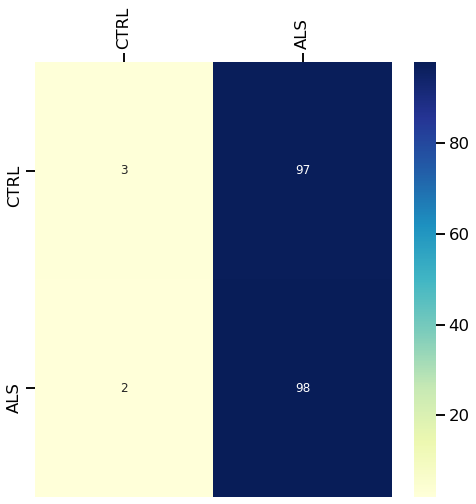
\includegraphics[width=8cm, height=8cm]{raw_model_results}
\end{figure}

Adding fine-tuning method described in the previous part to this model, an accuracy of 72.8\% is obtained. These results are shown by the confusion matrix below. (Figure 2)
\begin{figure}[H]
\centering
\caption{Confusion-matrix resulting from the pre-trained model, with fine-tuning method}
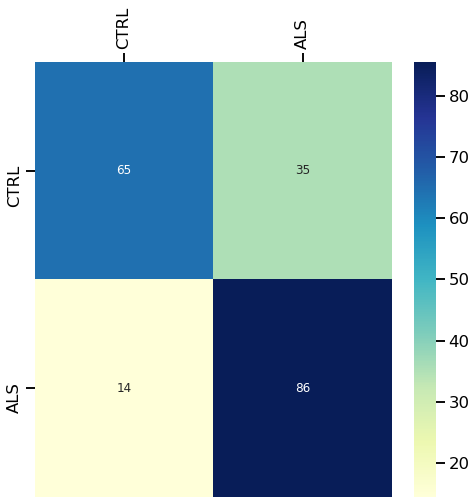
\includegraphics[width=8cm, height=8cm]{finetuning_model_results}
\end{figure}

When data augmentation is added to this method, the accuracy obtain is sligthly better, the accuracy is now 74.4\%. (Figure 3)
\begin{figure}[H]
\centering
\caption{Confusion-matrix resulting from the pre-trained model, with fine-tuning and data augmentation methods}
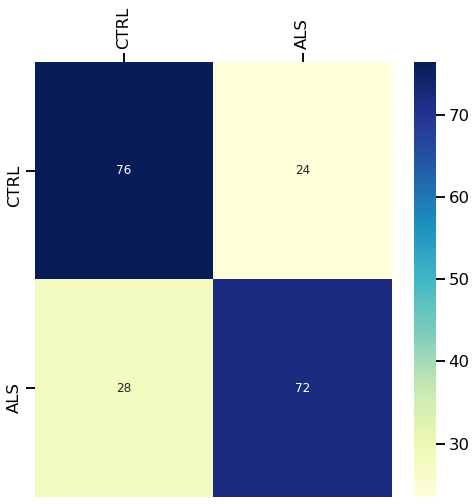
\includegraphics[width=8cm, height=8cm]{finetuning_data_augmentation_model_results}
\end{figure}

Regarding the features extraction, best results are obtained using the same pre-trained model and cuting the last block of it. The accuracy obtained is 72.6\% which is slightly lower than the one obtained with fine-tuning methods. This results is obtained using a Deep ML model as predictor, with classical models accuracy is better, but there is an overfitting problem. (Figure 4)
\begin{figure}[H]
\centering
\caption{Confusion-matrix resulting from the pre-trained model as features extractor}
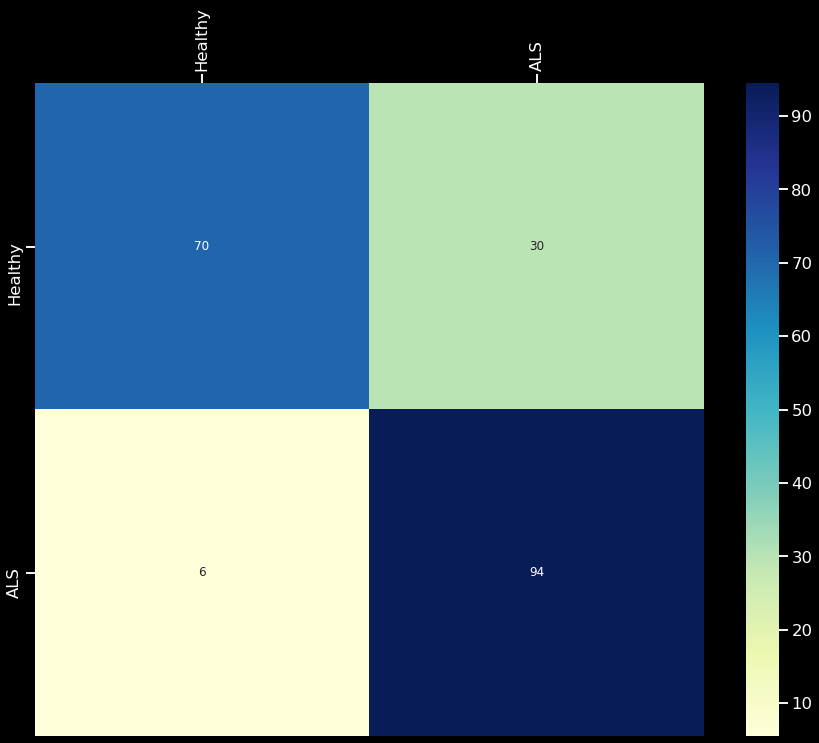
\includegraphics[width=8cm, height=8cm]{extractor_model_results}
\end{figure}

When data augmentation is applied to this model, the results are slightly improved. The accuracy obtained is 77\%. (Figure 5)
\begin{figure}[H]
\centering
\caption{Confusion-matrix resulting from the pre-trained model as features extractor, with data augmentation}
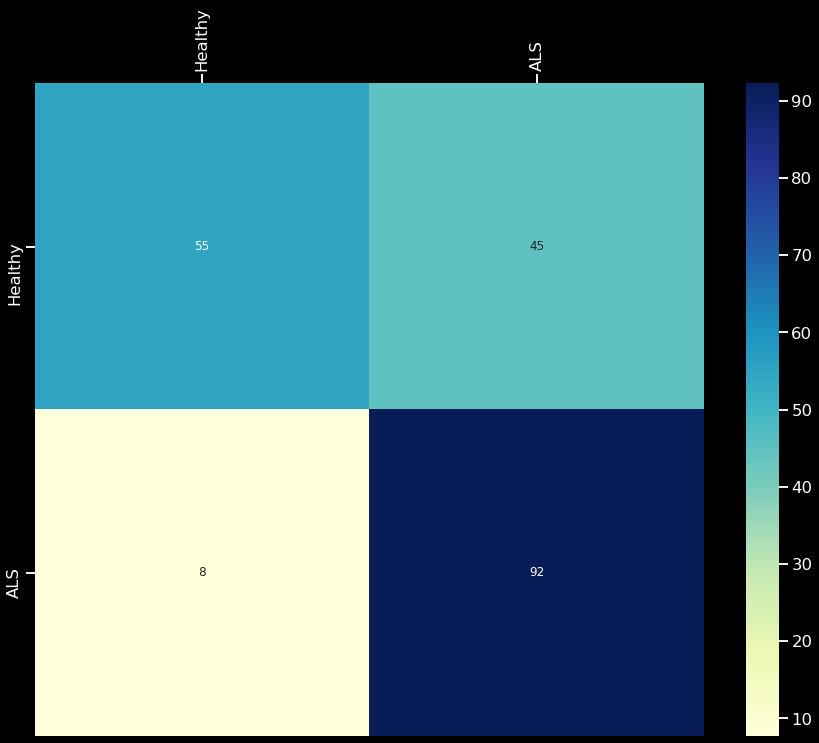
\includegraphics[width=8cm, height=8cm]{extractor_data_augmentation_model_results}
\end{figure}


\section{Discussion}
The discussion section aims at interpreting the results in light of the project's objectives. The most important goal of this section is to interpret the results so that the reader is informed of the insight or answers that the results provide. This section should also present an evaluation of the particular approach taken by the group. For example: Based on the results, how could the experimental procedure be improved? What additional, future work may be warranted? What recommendations can be drawn?


\section{Conclusions}
Conclusions should summarize the central points made in the Discussion section, reinforcing for the reader the value and implications of the work. If the results were not definitive, specific future work that may be needed can be (briefly) described. The conclusions should never contain ``surprises''. Therefore, any conclusions should be based on observations and data already discussed. It is considered extremely bad form to introduce new data in the conclusions.

\section{Data and code availability}
All the data and the code are available on \href{https://github.com/nsgln/Deep-Learning-Raman-Spectroscopy}{GitHub}

\begin{thebibliography}{9}
\bibitem{bacteria-ID} 
Ho, CS., Jean, N., Hogan, C.A. and al.
\textit{Rapid identification of pathogenic bacteria using Raman spectroscopy and deep learning}. 
Nat Commun 10, 4927 (2019).
\\\texttt{https://doi.org/10.1038/s41467-019-12898-9}

\bibitem{spectrum-recognition} 
Jinchao, L., Osadchy, M., Ashton, L., Foster, M., Solomon, C.J. and Gibson, Stuart J.
\textit{Deep convolutional neural networks for Raman spectrum recognition: a unified solution}.
Analyst, 142, 4067-4074 (2017).
\\\texttt{https://doi.org/10.1039/C7AN01371J}

\bibitem{data-augmentation} 
Bjerrum, E.J., Glahder, M. and Skov, T.
\textit{Data Augmentation of Spectral Data for Convolutional Neural Network (CNN) Based Deep Chemometrics}.
\\\texttt{https://arxiv.org/pdf/1710.01927.pdf}
\end{thebibliography}

\end{document}